% "Станет проще"

\documentclass[a4paper,12pt]{article} % тип документа

% report, book

% Рисунки
\usepackage{graphicx}
\usepackage{wrapfig}
\usepackage{hyperref}
\usepackage[rgb]{xcolor}



%  Русский язык

\usepackage[T2A]{fontenc}			% кодировка
\usepackage[utf8]{inputenc}			% кодировка исходного текста
\usepackage[english,russian]{babel}	% локализация и переносы


% Математика
\usepackage{amsmath,amsfonts,amssymb,amsthm,mathtools} 


\usepackage{wasysym}

%Заговолок
\author{Сафиуллин Роберт	}
\title{Лабораторная работа 3.6.1\\ СПЕКТРАЛЬНЫЙ АНАЛИЗ ЭЛЕКТРИЧЕСКИХ СИГНАЛОВ}





\begin{document} % начало документа

\maketitle


\newpage
\section{Цель работы:}
  В работе изучаются спектры периодических электрических сигналов
различной формы (последовательности прямоугольных импульсов и цугов,
а также амплитудно- и фазо-модулированных гармонических колебаний).
Спектры этих сигналов наблюдаются с помощью спектроанализатора, входящего
в состав USB-осциллографа и сравниваются с рассчитанными теоретически.
\\
\section{В работе используются:}
персональный компьютер; USB-осциллограф АКИП4107;
функциональный генератор WaveStation 2012; соединительные кабели.

 
\section{Экспериментальная установка:}

 \includegraphics[scale=0.6]{3611}
\section{Ход работы}
1) Проанализируем как меняетсяя спектр при изменении параметров $\Delta$$\nu$ и $f_povt$




















































































1) Cобрали схему и включили приборы\\
2) Рассчитали резонансную частоту по формуле: $\nu_0$=1/2$\pi$$\sqrt{LC}$=1592 Гц  (емкость конденсатора - 0.1 мкФ)\\
3) Сделав отклонения в обе стороны от $\nu_0$ снимем показания напряжения при разных значениях R. \\ 
Результаты запишем в таблицу и построим по ним график:


\begin{flushleft}

\begin {tabular}{|c|c|c|c|c|c|c|c|c|c|c|c|}
\hline 
\multicolumn{12}{|c|}{R=0 $\Omega$     }  \\ 
\hline 
$\nu$, Гц & 1588 & 1534 & 1580 & 1575 & 1582 & 1566 & 1592 & 1590 & 1605 & 1667 & 1698  \\ 
\hline 
U, В& 1.31 & 0.77 & 1.26 & 1.22 & 1.24 & 1.15 & 1.44 & 1.35 & 1.27 & 0.87 & 0.66  \\ 
\hline 
$\nu$/$\nu_0$ & 0.997 & 0.963 & 0.992 & 0.989 & 0.993 & 0.983 & 1 & 0.998 & 1.008 & 1.047 & 1.066  \\ 
\hline 
U/$U_0$ & 0.909 & 0.534 & 0.875 & 0.847 & 0.861 & 0.799 & 1 & 0.9375 & 0.882 & 0.604 & 0.458  \\ 
\hline 
\multicolumn{12}{|c|}{R=100 $\Omega$     }  \\  
\hline 
$\nu$, Гц & 1592 & 1630 & 1663 & 1693 & 1722 & 1526 & 1460 & 1488 & 1433 & • & •  \\ 
\hline 
U, В & 0.75 & 0.66 & 0.6 & 0.54 & 0.45 & 0.66 & 0.45 & 0.57 & 0.36 & • & • \\ 
\hline 
$\nu$/$\nu_0$ & 1 & 1.023 & 1.044 & 1.063 & 1.08 & 0.958 & 0.917 & 0.935 & 0.9 & • & •  \\ 
\hline 
U/$U_0$ & 1 & 0.88 & 0.8 & 0.72 & 0.6 & 0.88 & 0.6 & 0.76 & 0.48 & • & • \\ 
\hline 
\end{tabular} 
\end{flushleft}






\begin{center}


\begin {tabular}{|c|c|c|}
\hline 
\multicolumn{3}{|c|}{R=0 $\Omega$     }  \\ 
\hline 
$\nu$, Гц & 1756 & 1652 \\ 
\hline 
U, В&  0.45 & 0.96 \\ 
\hline 
$\nu$/$\nu_0$  & 1.1 & 1.04 \\ 
\hline 
U/$U_0$ &  0.31 & 0.66 \\ 
\hline 
\multicolumn{3}{|c|}{R=100 $\Omega$     }  \\  
\hline 
$\nu$ & • & • \\ 
\hline 
U &  • & • \\ 
\hline 
$\nu$/$\nu_0$ &  • & • \\ 
\hline 
U/$U_0$ &  • & • \\ 
\hline 
\end{tabular} 
\end{center}







\begin{flushleft}
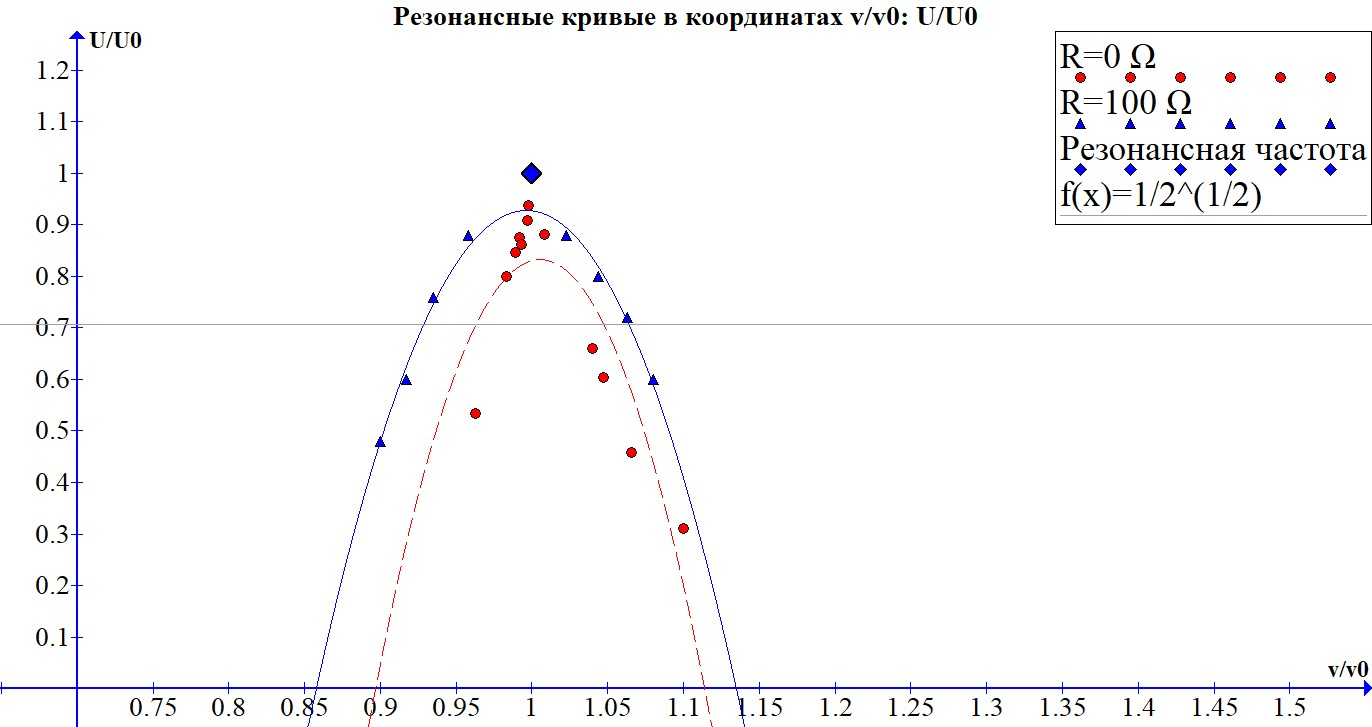
\includegraphics[scale=0.35]{3251}\\
\end{flushleft}        
 Определим  $Q_{graf}$ , рассчитав ширину кривых при значении ординаты  $\frac{1}{\sqrt[ ]{2}}$ и использовав формулy: $Q=\frac{\omega_0}{\Delta\Omega}$ \\
 
4) Подключим контур к клемме "Цуги" и установим резонансную частоту.\\
5) Измерим значения амплитуд для R=0 $\Omega$ и R=100 $\Omega$.\\
Результаты запишем в таблицу:

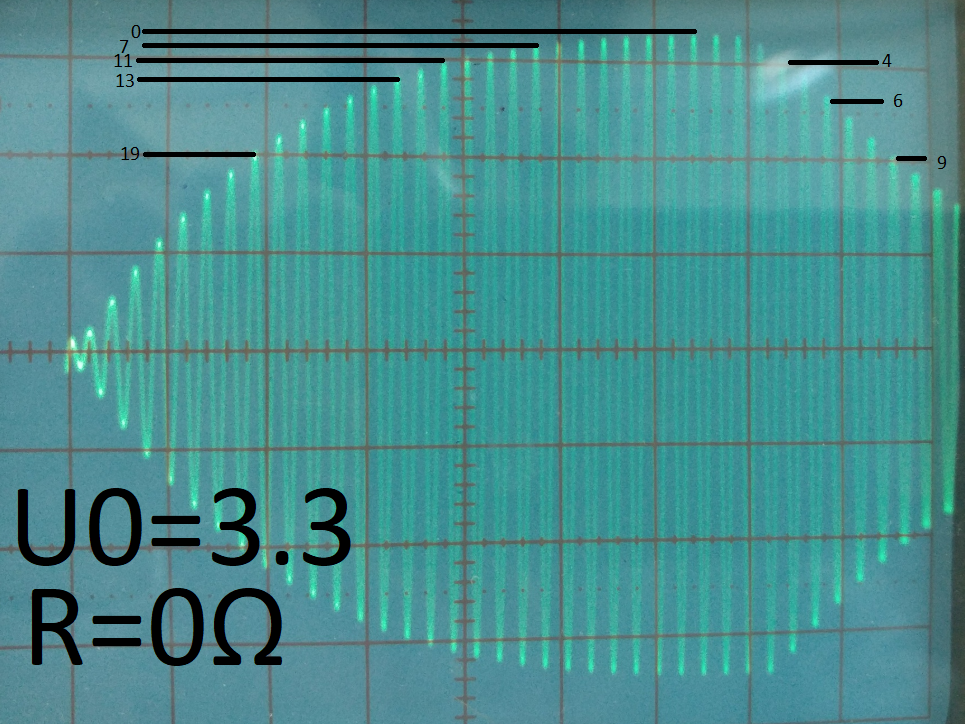
\includegraphics[scale=0.6]{r100}\\

\begin{tabular}{|c|c|c|c|c|c|c|}
\hline 
• &\multicolumn{2}{|c|}{1} & \multicolumn{2}{|c|}{2} & \multicolumn{2}{|c|}{3} \\ 
\hline 
$R_0^{ubivanie}$ &$U_{0+4}$=3.0 & $U_{0+9}$=2.0 & $U_{0+6}$=2.5 & $U_{0+13}$=1.4 & $U_{0+6}$=2.5 & $U_{0+17}$=1.0 \\ 
\hline 
$R_0^{vozrastanie}$ &$U_{0+7}$=3.2 & $U_{0+11}$=3.0 & $U_{0+13}$=2.8 & $U_{0+10}$=3.0 & $U_{0+21}$=1.6 & $U_{0+19}$=2.0 \\ 
\hline 

\end{tabular} 

\begin{center}





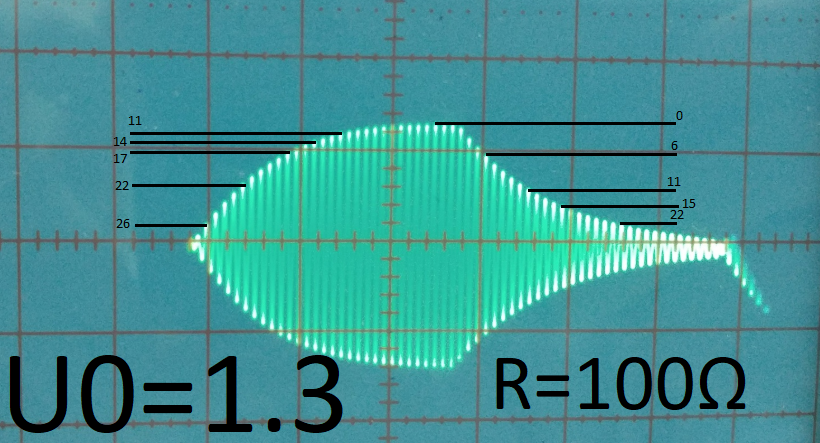
\includegraphics[scale=1.0]{r0}\\
\end{center}			
\begin{tabular}{|c|c|c|c|c|c|c|}
\hline 
• &\multicolumn{2}{|c|}{1} & \multicolumn{2}{|c|}{2} & \multicolumn{2}{|c|}{3} \\ 
\hline 
$R_{100}^{ubivanie}$ &$U_{0+6}$=1.0 & $U_{0+11}$=0.6 & $U_{0+15}$=0.4 & $U_{0+6}$=1.0 & $U_{0+22}$=0.2 & $U_{0+15}$=0.6 \\ 
\hline 
$R_{100}^{vozrastanie}$ &$U_{0+11}$=1.2 & $U_{0+17}$=1.0 & $U_{0+14}$=1.1 & $U_{0+22}$=0.6 & $U_{0+26}$=0.2 & $U_{0+17}$=1.0 \\ 
\hline 

\end{tabular}  \\

6) Рассчитаем по ним добротность Q с помощью формулы:\\
\begin{equation} 
Q=\frac  {\pi}   {   \frac{\ln{\frac{U_0-U_{0+k}}{U_0-U_{0+k+n}}}}{n}    }    
\end{equation}
\\
\begin{center}

\begin{tabular}{|c|c|c|c|c|}
\hline 
• & 1 & 2 & 3 & Среднее \\ 
\hline 
$Q^{ubivanie}_0$ & 10.71 & 25.42 & 32.7 & 23$\pm$9.3 \\ 
\hline 
$Q^{vozrastanie}_0$ & 11.43 & 5.43 & 23.42 & 13.42$\pm$7.5 \\ 
\hline 
$Q^{ubivanie}_{100}$ & 18.53 & 25.73 & 48.65 & 25.11$\pm$12\\ 
\hline 
$Q^{vozrastanie}_{100}$ & 17.57 & 20.96 & 21.8 & 19.7$\pm$1.7 \\ 
\hline 
\end{tabular}  

\end{center}
 Теоретическое значение добротности по параметрам контура: \\
\begin{equation}
Q_0=\frac{1}{R} *\sqrt[] {\frac{L}{C}}=42.55             
\end{equation}\\
\begin{equation}
Q_{100}=\frac{1}{R} *\sqrt[] {\frac{L}{C}}=8.1
\end{equation}

7) Получим картину биений. Их появление связано с тем, что разность фаз двух близких по частоте колебаний медленно меняется
\begin{center}

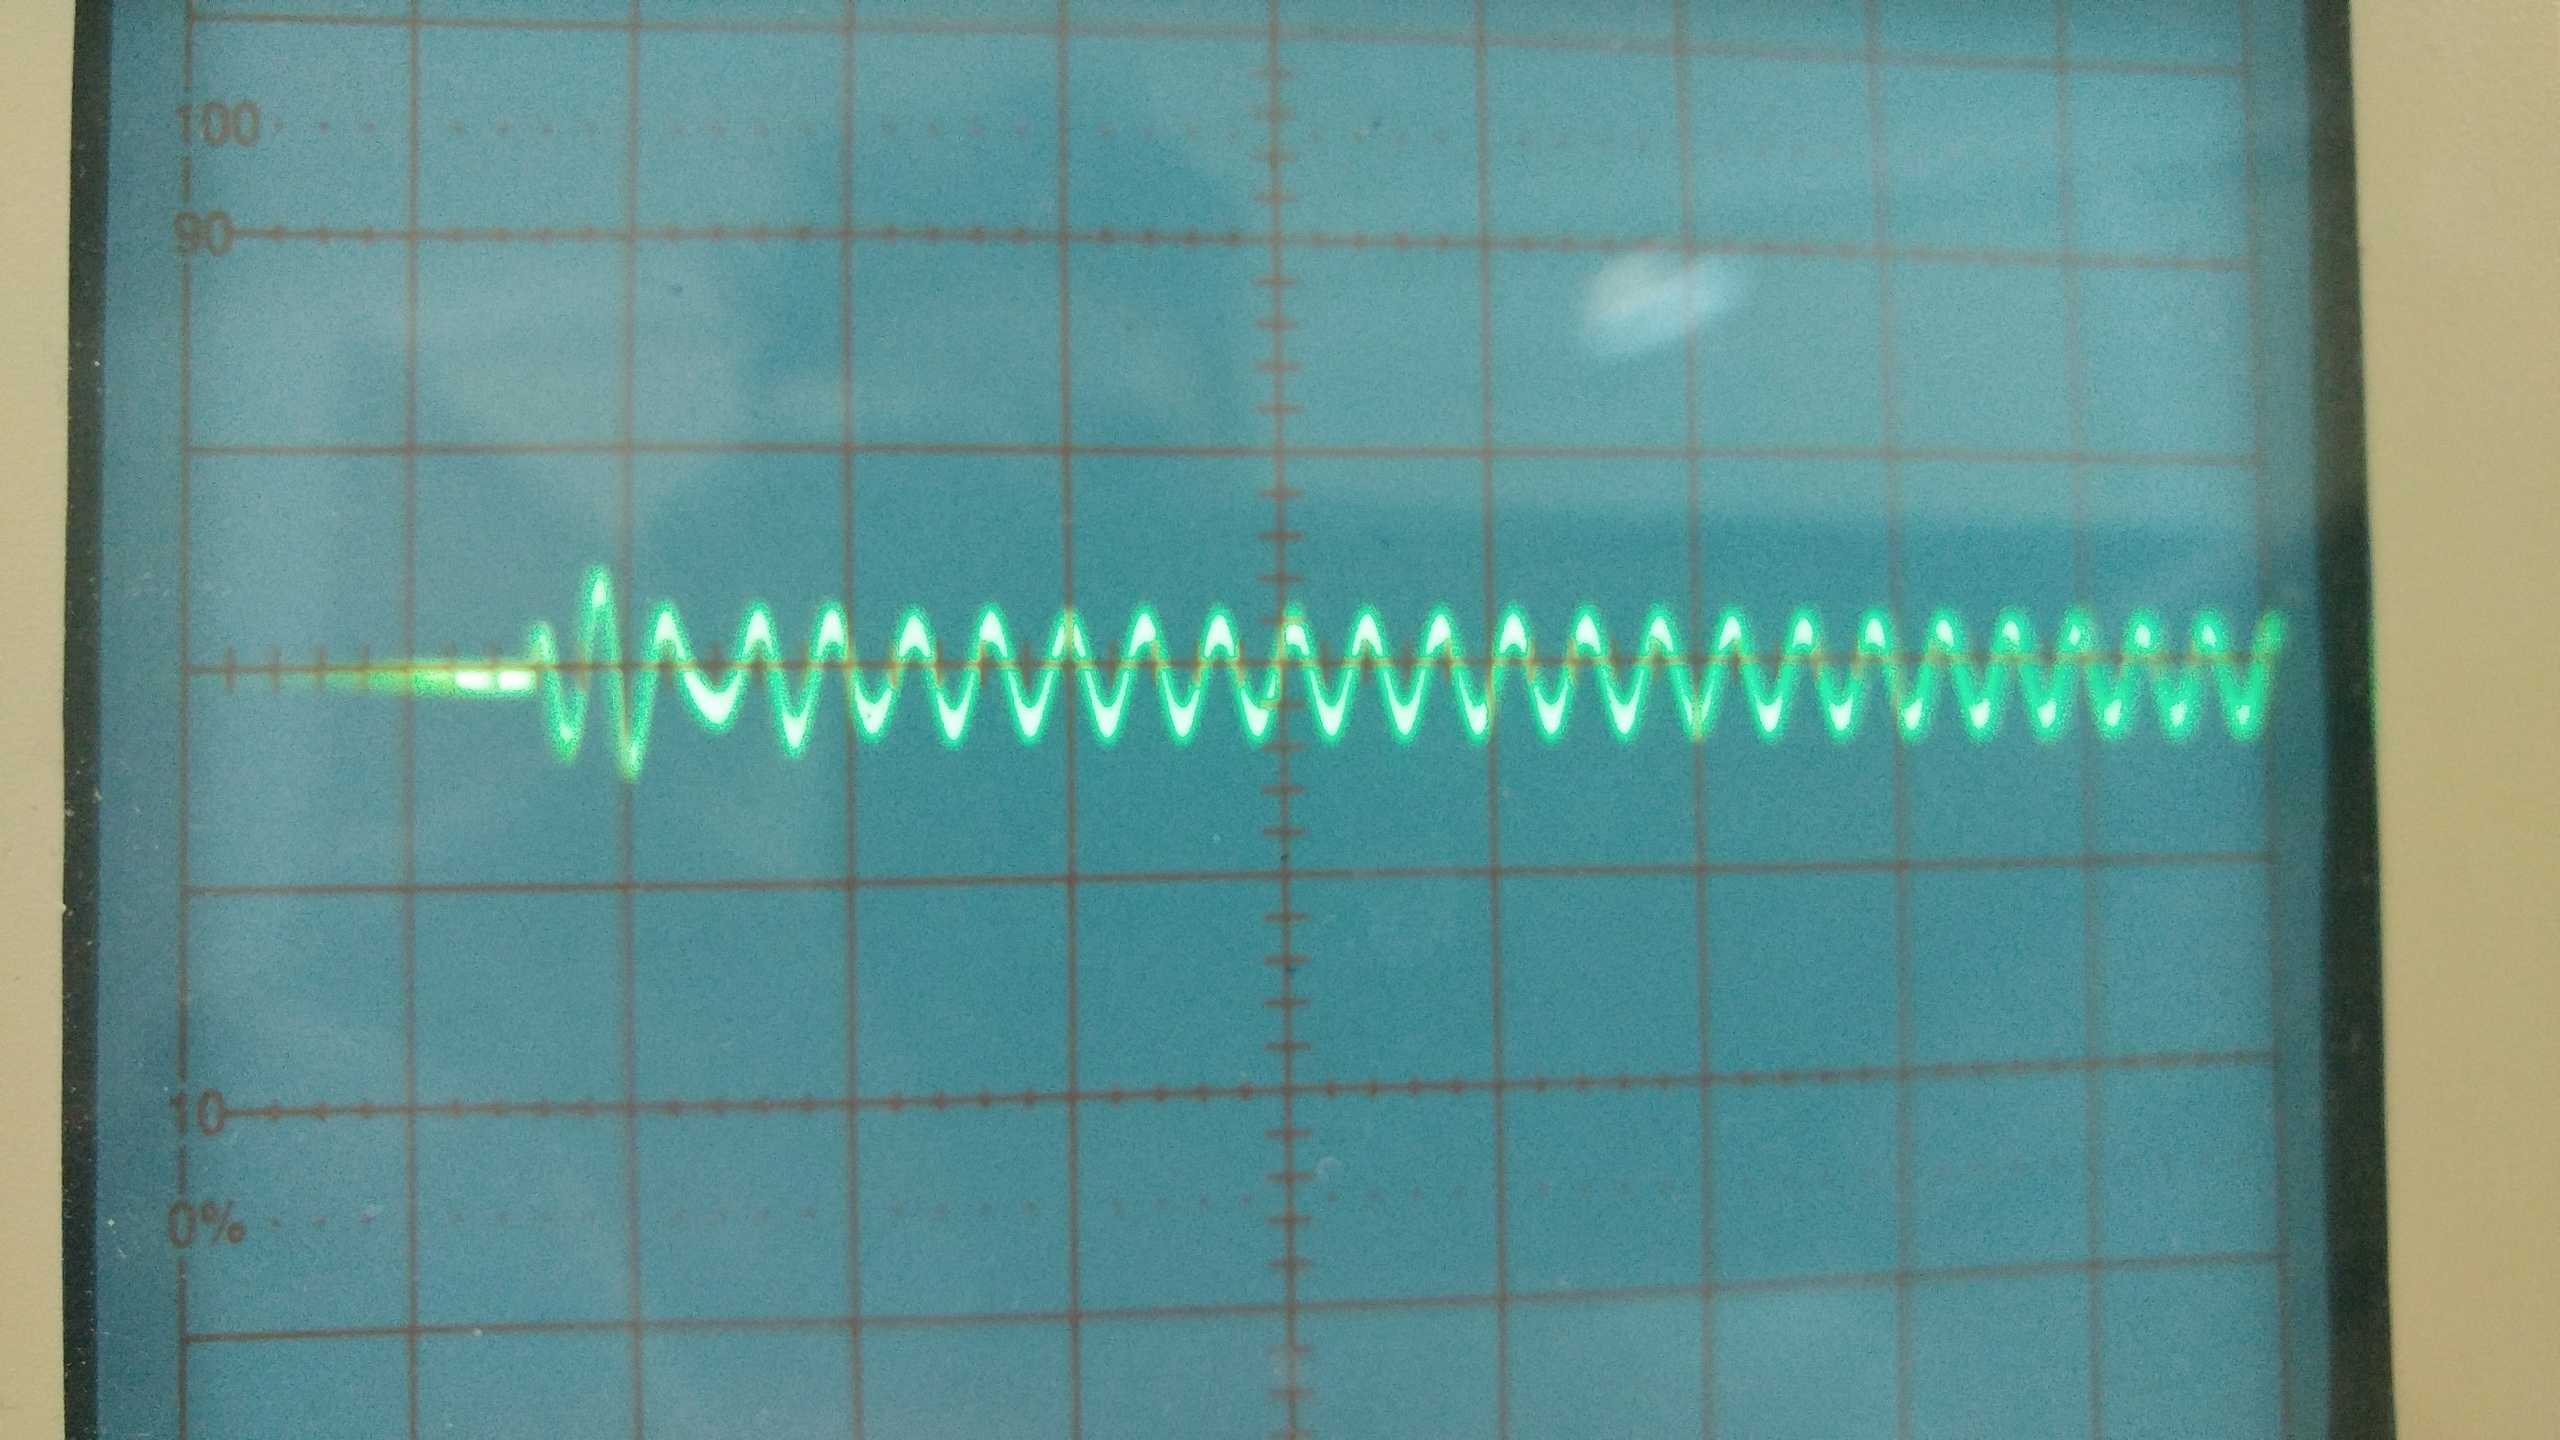
\includegraphics[scale=0.1]{bi}\\
\end{center}
 
8) Проведем измерения на мосте переменного тока и результаты занесем в таблицу: \\
\begin{center}


\begin{tabular}{|c|c|c|}
\hline 
$\nu$, Гц & L, мГн & R,$\Omega$ \\ 
\hline 
50 & 99.967 & 26.36 \\ 
\hline 
500 & 100 & 22.49 \\ 
\hline 
1500 & 100 & 23.5 \\ 
\hline 
\end{tabular} 
\end{center}	 
8) Cведем все найденные добротности в таблицу: \\
\begin{center}
\begin{tabular}{|c|c|c|c|c|c|}
\hline 
R, $\Omega$ & $R_{kont}$, $\Omega$ & $Q_{graf}$ & $Q_{vozr}$ & $Q_{ubiv}$ & $Q_{LCR}$ \\ 
\hline 
0 & 23.5 & 12 & 13.4$\pm$7.5 & 23$\pm$9.3 & 42.5 \\ 
\hline 
100 & 123.5 & 7.24 & 19.7$\pm$1.7 & 31$\pm$12 & 8.1 \\ 
\hline 
\end{tabular} 

\end{center}























\end{document} % конец документа
